\begin{frame}{Data from CSV File}
\begin{center}
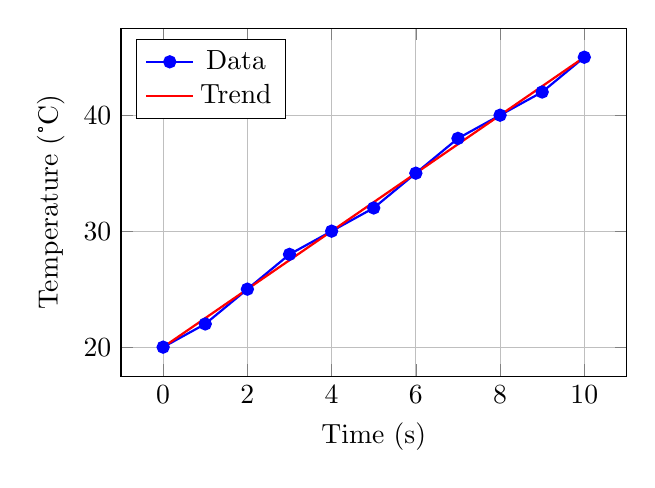
\begin{tikzpicture}
\begin{axis}[
    xlabel={Time (s)},
    ylabel={Temperature (°C)},
    grid=both,
    width=8cm,
    height=6cm,
    legend pos=north west
]
% Simulated data points
\addplot[thick, blue, mark=*, mark size=2pt] coordinates {
    (0,20) (1,22) (2,25) (3,28) (4,30) (5,32) (6,35) (7,38) (8,40) (9,42) (10,45)
};
\addplot[thick, red, domain=0:10] {20 + 2.5*x};
\legend{Data, Trend}
\end{axis}
\end{tikzpicture}
\end{center}

\footnotesize
\texttt{\textbackslash addplot[thick, blue, mark=*, mark size=2pt] coordinates \{\}}
\end{frame}